\section{Design}
\label{sec:design}
\sys{} coordinates readiness during data upload and generates destination completion notifications on the managed network path. This section describes those operations and the resource contracts they require.

\subsection{Overview and Assumptions}
\label{sec:overview}
Figure~\ref{fig:design-overview} contrasts the baseline with our two changes: uploading during readiness aggregation and appending completion notifications to trailing data.
\begin{figure*}[t]
\centering
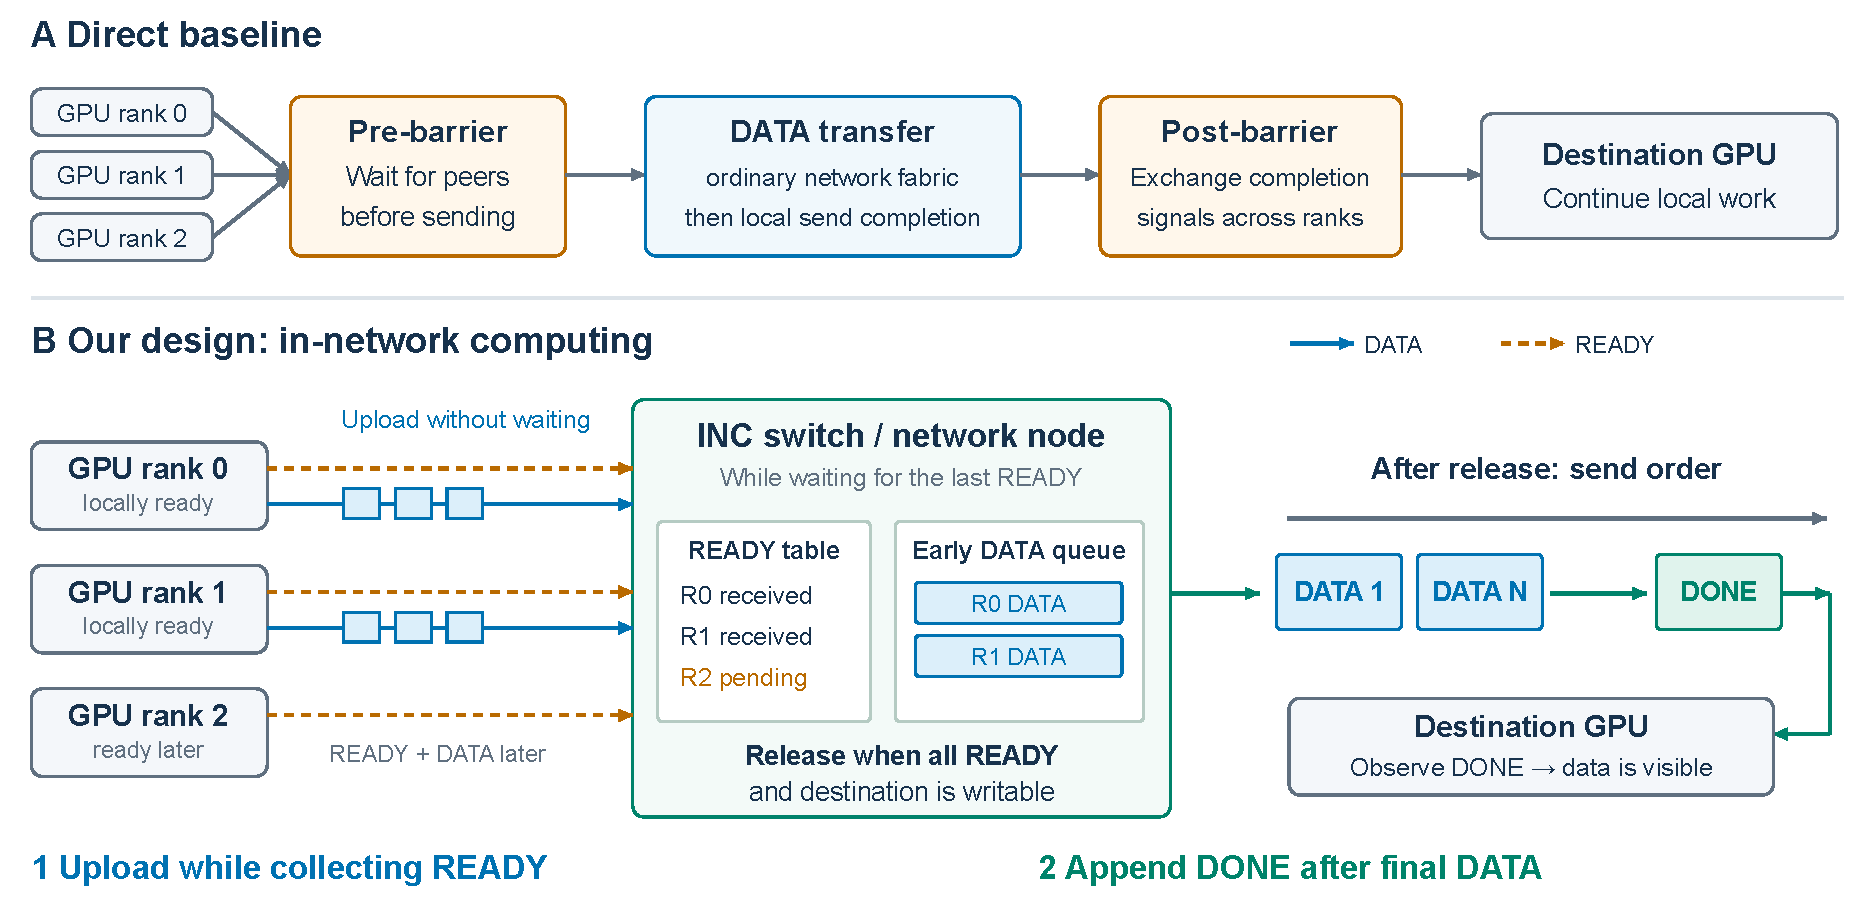
\includegraphics[width=\textwidth]{figures/inc-overview.pdf}
\caption{Two changes to Direct coordination: upload data while collecting READY, then append ordered DONE after the destination's final data. The queue shows the waiting stage; the right-hand sequence shows transmission after forwarding starts. Destination writability, data visibility, and buffer-lifetime requirements remain.}
\Description{The Direct baseline serializes pre-barrier, data transfer and sender completion, and post-barrier. With INC, ranks zero and one upload while rank two is not yet ready. The network stores READY state and early data. Once all ranks are ready, it sends data followed by DONE to the destination.}
\label{fig:design-overview}
\end{figure*}

The logical \sys{} node observes all readiness announcements and data covered by its completion decisions. For each generation it maintains (i) a participant bitmap, (ii) sealed per-destination traffic plans, (iii) output progress, (iv) destination memory descriptors, and (v) bounded staging. A generation identifies the communication instance, direction, and buffer epoch. The EP membership is known; routing determines the per-destination traffic. We assume reliable delivery with an ordering guarantee: data covered by \done{} is visible in GPU memory before \done{} is observed.

Before upload, the source obtains admission to network staging. Each destination publishes its reserved staging region, capacity, access rights, and epoch. Staging addresses must be resolvable without global receive counts, for example using a source-reserved region and a per-destination record ordinal. Each token carries its routing information and record identity, allowing INC to determine its destinations and staging positions as it arrives. Compact expert placement can be computed separately.

All traffic counted by the node must pass through its observation and completion domain. With multiple rails or nodes, progress must be partitioned and joined explicitly. Any local bypass requires a separate completion check at the consumer. The single-node measurements in Section~\ref{sec:e2e} are reference measurements; the design does not assume that an Ethernet node observes local NVLink traffic.

\subsection{Readiness Aggregation and Early Upload}
\label{sec:early-upload}
After routing and local preparation, source $s$ sends \ready{} together with a count vector: element $d$ gives its planned number of output records for destination $d$. It then uploads admitted \data{} without waiting for other ranks. INC marks a source ready only after accepting its complete vector; duplicate announcements are ignored. The node buffers early data and begins accumulating vectors as they arrive.

Once all required \ready{} messages have arrived and destination staging is writable, INC parses token routes and fans out buffered and arriving data, subject to output capacity. Vector accumulation proceeds in parallel and need not finish before fan-out starts. Thus, readiness receipt gates forwarding, while finalized counts gate completion notification. Local routing and count-vector construction remain source-side work.

The readiness dependency remains: the network cannot deliver into an unready destination. What changes is that the source-to-node transfer can proceed while readiness is being aggregated. The node's location permits this transfer to share the eventual data path. Whether the head start reduces operation latency depends on the slowest required source and the output queue, as analyzed in Section~\ref{sec:readiness-analysis}.

For Dispatch, global receive counts and final expert offsets can be computed alongside transfers into reserved staging. Count-vector entries must match the records actually emitted by fan-out, including any replication. Hardware can pipeline the integer additions with upload and forwarding; any remaining aggregation delay is included in completion latency. Multicast bandwidth savings are separate from the synchronization mechanism.

\subsection{Completion Notification}
\label{sec:completion-design}
For Dispatch generation $g$, the count vector from source $s$ contains $n_{g,s,d}$ unique output records for destination $d$. INC accumulates these vectors to obtain
\begin{equation}
 N_{g,d}=\sum_s n_{g,s,d}.
 \label{eq:count}
\end{equation}
The expected count becomes valid only after every required source has supplied its complete vector and all additions have finished. A zero entry explicitly reports no traffic; silence does not. Planned counts and output progress use the same record unit, with a fragmented record counted only when all its fragments have been submitted. Input packets, multicast replicas, and reduced outputs require their own accounting.

The node appends \done$(g,d)$ only when $N_{g,d}$ is valid and all $N_{g,d}$ records have entered the appropriate ordered delivery channel. If data finishes first, DONE waits for the final count; a destination with zero expected records is notified once its count is valid and it is ready. At the receiver, the required contract is
\begin{equation}
 \operatorname{observe}_d(\done(g,d))
 \Rightarrow
 \bigwedge_{x\in\mathcal{D}_{g,d}}\operatorname{visible}_d(x),
 \label{eq:visible}
\end{equation}
where $\mathcal{D}_{g,d}$ is the complete expected input. Output progress determines when a notification may be generated; the transport and receiver must separately establish this visibility implication.

NCCL GIN's strong-signal ordering applies to preceding PUTs to the same peer on the same context~\cite{gindocs}. A network-generated notification needs an equivalent delivery contract. Separate contexts or rails require a join, and a subsequent local forwarding hop requires its own visibility check. The distinction is about the ordering domain, not simply whether communication is within or across nodes.

Reliable delivery and duplicate suppression must precede logical progress accounting. Retransmitted fragments must not make a counter reach its target while another fragment is missing.

\done$(g,d)$ proves completion for destination $d$, rather than completion of all consumers in the EP group. A successor can use it only when destination-local completion, layout readiness, and the remaining local dependencies are sufficient. Applications that require a genuine global join retain it.

For Combine, the token owner establishes the expected contributor set during Dispatch. Contributions are identified by route slot, since several experts can occupy the same rank. Producers send weighted partials; an existing in-network reduction mechanism accumulates the expected fragments and produces the result~\cite{dysharp,switchml}. The node separately tracks input-contribution completion and reduced-output completion before notifying the owner. We attribute neither the arithmetic mechanism nor its bandwidth benefit to the synchronization design.

\subsection{Buffer Management and Progress}
\label{sec:resources}
A destination's readiness announcement commits its receive slot to the current epoch until the generation has finished using it. After observing \done{} and satisfying local requirements, Dispatch can compact the received records for expert computation; Combine can release the reduced result to its consumer. The last consumer then publishes \recycle{} and permits reuse. Emitting \done{} alone never permits overwrite.

The sender also retains its source buffer until the transport has finished reading it. Generating target notification in the network decouples the target's release from the sender's completion path; it does not remove source-lifetime tracking. Different generations therefore require separate ownership state.

Network capacity covers early arrivals, input/output imbalance after release, and any reduction accumulators. Admission must respect this capacity. When space is exhausted, unadmitted data waits at the source and continues on the same path when resources become available.

Control messages need guaranteed progress: a full data queue must not block the \ready{} messages needed to release it. Reserved control resources or an equivalent queue separation are required. PFC may provide link-level protection~\cite{pfc}, but its use does not remove the need for headroom, admission, and deadlock analysis. Capacity pressure can reduce overlap or throughput. Recovery from endpoint or network-node failure is outside the assumed reliable-delivery model.
